\chapter{IoT-Security}
In diesem Kapitel sollen wichtige Aspekte der Security im IoT-Umfeld erarbeitet werden. Verschiedene Bereiche in der Architektur und deren Herausforderungen bezüglich Security erfordern unterschiedliche Massnahmen. Es wird versucht, zentrale Aspekte hervorzuheben, eine umfassende Behandlung ist in diesem Rahmen jedoch nicht möglich.
\section{Einführung}
Sicherheit ist im IoT-Bereich in den letzten Jahren immer wichtiger geworden. Viele Hersteller wollen ihre Produkte schnellstmöglich auf den Markt bringen und beachten Sicherheitsanforderungen zu wenig. Laut einer Studie von HP kamen bei den meisten Produkten schwerwiegende Sicherheitsbedenken auf.\cite{SecOverview} 

Die Vielfalt an Geräten bringt eine grosse Angriffsfläche mit sich. Verantwortliche müssen bei jedem Hersteller umfassende Sicherheitsanalysen durchführen. Im Gegensatz zu traditionellen Firmennetzwerken sind Netzwerke mit IoT-Devices schwieriger abzusichern. Bisher haben fast ausschliesslich Menschen die Kommunikation in Netzwerken verursacht. Maschine-zu-Maschine (M2M) Kommunikation ist in IoT-Netzwerken zentral. Menschen kommunizieren nur in seltenen Fällen (Konfiguration, Fehlerbehandlung, etc.) direkt mit den End-Devices. Die IoT-Devices haben dennoch ständige Kommunikation über das Netzwerk oder gar das Internet. Eine Kompromittierung dieser Systeme ist also theoretisch möglich.

\subsection{Folgen}
Die Vergangenheit hat gezeigt, dass Sicherheitsvorfälle schwerwiegende Folgen haben können. Reputationsverluste, Datenverluste, Industriespionage oder Systemausfälle durch Denial-of-Service (DoS) können Unternehmen beträchtlichen finanziellen Schaden zufügen. Wie seit einigen Jahren bekannt ist, haben selbst Regierungen von Weltmächten wie China, Russland oder die USA Interesse an der illegalen Beschaffung von Daten und Informationen. Die Motivation und technischen Fähigkeiten von Angreifern auf IT-Systeme sind sehr unterschiedlich. Ebenso unterscheiden sich die Sicherheitsbedürfnisse von Unternehmen stark.

Durch Entwicklungen im IoT-Umfeld muss damit gerechnet werden, dass IT-Systeme noch viel weiter als heute in Unternehmensprozessen eingebunden werden. Mit der Vision der Industrie 4.0 werden ganze Geschäftsprozesse vollautomatisiert und manuelle Tätigkeiten werden weitestgehend eliminiert. Wenn man von automatisierten Produktionsstätten ausgeht, kommen einige Gefahren zum Vorschein. Die Konkurrenz könnte beispielsweise durch gezielte Attacken auf ein Fertigungssystem Fehler einprogrammieren, welche zu grossen Rückrufaktionen und Reputationsverlusten führen könnten. Nochmals eine Stufe gefährlicher sind Attacken, welche Leib und Leben gefährden können. Denkt man an den medizinischen Bereich, könnten Patientensysteme, welche für die Medikation von Patienten zuständig sind, übernommen werden.

Es ist also ersichtlich, dass zu den herkömmlichen finanziellen Schäden bei IoT-Systemen Gefährdungen für Leib und Leben existieren können. Gesetzgeber wie auch Ingenieure müssen sich mit diesen wichtigen Herausforderungen intensiv befassen.

\subsection{Grobübersicht}  
Um eine möglichst übersichtliche Vorstellung von IoT-Security zu erhalten, werden vier grobe Architekturbereiche einzeln behandelt. Jeder dieser Bereiche birgt eigene Gefahren und benötigt unterschiedliche Massnahmen um die Informationssicherheit zu gewährleisten.
\begin{figure}[H]
\centering
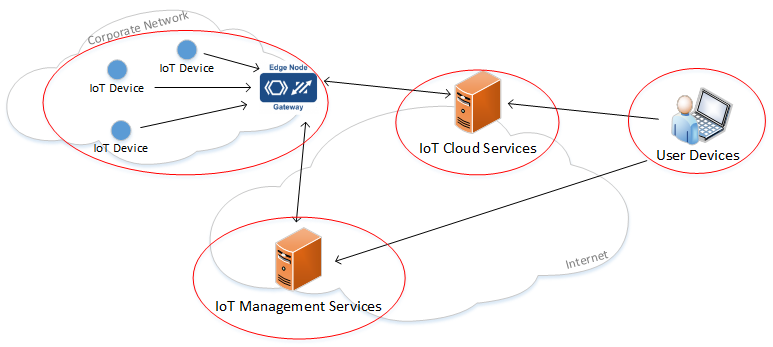
\includegraphics[scale=0.8]{../02_Analyse/images/security_overview.png}
\caption{Sicherheitszonen}
\end{figure}
\subsubsection{Device-Networks}
Device-Netzwerke beinhalten die IoT-Devices. Diese können sehr unterschiedlich aussehen. Denkbar wären Wireless Sensor Netzwerke (WSN), es könnten aber auch ''herkömmliche'', verkabelte Netzwerke sein. Die Heterogenität ist sehr gross, da nicht nur viele unterschiedliche Hersteller existieren, sondern auch die Arten der Kommunikation und die verwendeten Protokolle sich unterscheiden. 

\subsubsection{IoT-Cloud-Services}
IoT-Devices selbst kommunizieren häufig über Cloud-Services im Internet. Entweder stellen die Hersteller der Devices selbst Cloud-Services zur Verfügung, oder die Unternehmen entwickeln eigene Applikationen. Auf der einen Seite kommunizieren die Server mit den IoT-Devices oder deren Gateways, auf der anderen Seite werden die Services von End-Usern selbst benutzt. Sensordaten könnten auch über bereitgestellte APIs von anderen Cloud-Services konsumiert werden.

\subsubsection{User-Devices}
Benutzer selbst kommunizieren in den seltensten Fällen direkt mit IoT-Devices sondern über bereitgestellte Cloud Dienste. Häufige Devices sind PCs, Laptops und Mobilgeräte wie Smartphones oder Tablets.

\subsubsection{IoT-Management-Services}
Unternehmen möchten ihre IoT-Devices über einen zentralen Service verwalten. Häufig liefern Hersteller eigene Management Software, diese beschränken sich aber oft auf die Verwaltung von Geräten derselben Hersteller.
\newpage
\section{Informationssicherheit}
Nach dem Parker'schen Hexad befasst sich die Informationssicherheit grundlegend mit sechs Bereichen: \cite{ParkerianHexad}
\subsubsection{Vertraulichkeit (Confidentiality)}
Die Information muss geheim bleiben und darf von Unbefugten nicht einsehbar sein. Die Vertraulichkeit werden zum einen mittels kryptografischen Funktionen sichergestellt, zum anderen durch Berechtigungen. Informationen werden verschlüsselt, die vorgesehenen Entitäten sind im Besitz der Schlüssel um an die Informationen zu gelangen. Verschlüsseln von Informationen wird seit Tausenden von Jahren verwendet. Es existieren unterschiedliche Algorithmen und Schlüssellängen. Verwendete Techniken sollten regelmässig auf deren Aktualität und Sicherheit überprüft werden.
\subsubsection{Besitz oder Kontrolle (Possession or Control)}
Wenn ein Unbefugter in den Besitz oder die Kontrolle der Information bekommt so muss nicht zwangsweise die Vertraulichkeit verletzt sein. Wird beispielsweise ein Laptop oder eine Kreditkarte gestohlen, so erhält der Dieb diesen Zugriff, obwohl er nie vorgesehen wurde. Um sich vor diesen Gefahren zu schützen, empfiehlt sich eine Multi-Faktor Authentisierung, bei der Besitz und geheimes Wissen benötigt wird. 
\subsubsection{Integrität (Integrity)}
Bei der Einhaltung der Integrität möchte man die unbefugte oder unbemerkte Veränderung der Daten verhindern. Integritätschecks werden meistens mit kryptografischen Hashfunktionen durchgeführt. Dabei wird mittels einer mathematischen Einwegfunktion ein sogenannter Hashwert einer Eingangsinformation erstellt. Dieser Hashwert ist praktisch einmalig und schwierig reproduzierbar, weshalb bei einer Veränderung der Eingangsinformation ein anderer Hashwert resultiert. 
\subsubsection{Echtheit (Authenticity)}
Die Echtheit einer Information ist in vielen alltäglichen Bereichen wichtig. So möchte man sicherstellen, dass eine erhaltene Rechnung auch wirklich von der Firma stammt, von welcher man die Leistung bezogen hat. Bei E-Mails und dem zugrunde liegenden SMTP-Protokoll sind Probleme der Authentizität vielen Personen bekannt. Die Kryptografie hat Verfahren für digitale Signaturen hervorgebracht. Mit einem geheimen Schlüssel kann eine Information signiert werden, der dazugehörige öffentliche Schlüssel dient zur Verifikation der signierten Nachricht.
\subsubsection{Verfügbarkeit (Availability)}
Die Sicherheit ist ebenfalls nicht gewährleistet, wenn Informationen nicht verfügbar sind. Durch Denial-of-Service (DoS) Attacken, aber auch durch schlechte Planung oder unvorhergesehenen Ausfällen können Verfügbarkeitsprobleme auftreten. Durch Hochverfügbarkeitscluster können Ausfälle einzelner Knoten aufgefangen werden und die Wahrscheinlichkeit von Ausfällen drastisch reduziert werden.
\subsubsection{Nützlichkeit (Utility)}
Als Beispiel für die Verletzung dieses Aspekts kann man sich am besten ein vergessenes Passwort vorstellen. Sämtliche anderen Sicherheitsaspekte sind erfüllt, die Information ist trotzdem nicht zugänglich, da der benötigte Schlüssel (das Passwort) fehlt. Solche Fälle können durch Key-Recovery Mechanismen abgefangen werden. \cite{ParkerianHexadWiki}
\section{Device-Networks}
In diesem Unterkapitel werden Gefahren und Herausforderungen in Netzwerken mit IoT-Devices beschrieben.
\subsection{Device-Security}
\subsubsection{Software Versionen}
Ein wichtiger Aspekt für Unternehmen ist die Aktualität der verwendeten Software Versionen auf ihren IoT-Devices. Wie heute üblich, wird Software oft unfertig, mit Bugs und fehlenden Features ausgeliefert. Nach der Installation muss also schon fest mit kommenden Updates gerechnet werden. Die Unternehmen müssen also über ihre Softwarestände in den IoT-Systemen im Bilde sein und über die Möglichkeit von zeitnahen Updates verfügen. 

\subsubsection{Physischer Zugriff}
Wie bei vielen anderen Geräten sollte auch bei IoT-Devices der physische Zugang nur autorisierten Personen vorbehalten sein. Sonst könnte beispielsweise ein Sensor manipuliert werden, der falsche Daten liefert.

\subsubsection{Authentifizierung und Autorisierung}
Da ein IoT-Device über das Internet kommuniziert, sollten Zugriffe authentifiziert und autorisiert werden. Durch unbefugten Zugriff können entweder potenziell sensible Sensordaten gelesen werden. Ausserdem besteht die Möglichkeit, einem Botnetz beizutreten, was mit geschützten Zugriffen teilweise entschärft werden kann. Es sollten ausserdem Mechanismen vorgesehen werden, welche zuständige Personen bei zu häufigen Fehlversuchen benachrichtigen, da potenziell eine Attacke vorliegen könnte.
 \newpage
\subsection{Netzwerksicherheit}
\subsubsection{Bootstrapping}
In der Bootstrapping-Phase betritt ein neues IoT-Device ein bestehendes Netzwerk. Eine Security-Association (SA) zwischen dem IoT-Device und dem Netzwerk, resp. deren Devices muss erstellt werden. Als Betreiber des Netzwerks muss man sicherstellen, dass nur vorgesehene Devices beitreten können, deshalb ist eine Authentisierung sehr wichtig. Das IoT-Device muss im Gegensatz dem Netzwerk vertrauen. Ein Server kann über Protokolle wie beispielsweise EAP neue Devices authentisieren.
\begin{figure}[H]
\centering
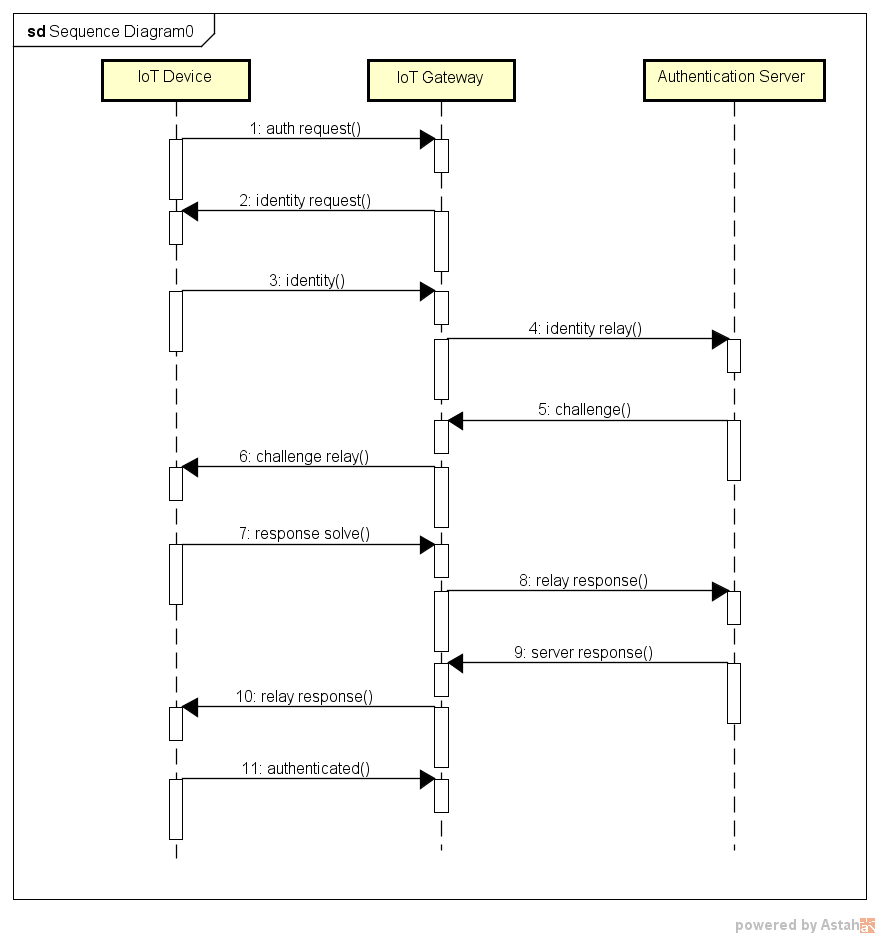
\includegraphics[scale=0.6]{../02_Analyse/images/deviceauthentication.png}
\caption{Schema möglicher Deviceauthentisierung}
\end{figure}
Im Gegensatz zu herkömmlichen Geräten, bei denen die Identität beispielsweise durch die Eingabe eines Passworts oder der Verteilung von Zertifikaten mittels einer PKI festgestellt werden kann, kommen bei IoT-Geräten erschwerende Hürden hinzu. \cite{IoTSecurityChallenges} So könnten Devices beispielsweise über keine direkten Eingabemöglichkeiten-, oder zu wenig Rechenleistung für herkömmliche asymmetrische Kryptografie verfügen.

\subsubsection{Verschlüsselung}
Weder das HTTP-, noch das CoAP-Protokoll haben eine eigene Verschlüsselung des Payloads vorgesehen. Seit langer Zeit wird für HTTP SSL, respektive TLS verwendet, um die Kommunikation zwischen zwei Devices zu verschlüsseln. TLS verschlüsselt die gesamten Pakete in der Applikationsschicht, Protokolle unterhalb der Applikationsschicht sind weiterhin im Klartext verfügbar. 

IoT-Devices arbeiten häufig mit CoAP anstatt HTTP. Wie in Kapitel \ref{sec:iotkomm} beschrieben, arbeitet CoAP im Gegensatz zu HTTP mit UDP anstelle von TCP. TLS selbst benötigt jedoch TCP als Transportprotokoll, weshalb sich dieses Verfahren also nicht für CoAP eignet.

Aus diesen Gründen musste ein neues Verschlüsselungsprotokoll DTLS (Datagram Transport Layer Security) entwickelt werden, welches ''TLS'' über UDP ermöglicht. Die Unterschiede von TLS zu DTLS sind gering. Einfach betrachtet erledigen die Protokolle die gleichen Aufgaben.

\begin{figure}[H]
\centering
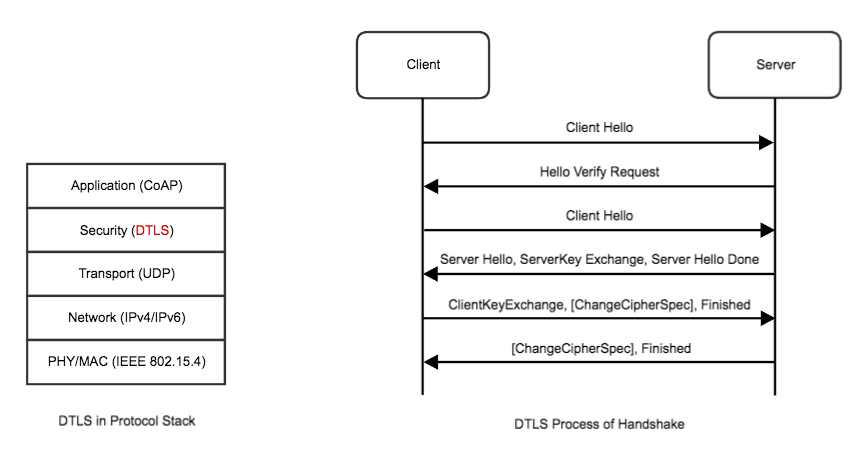
\includegraphics[scale=0.5]{../02_Analyse/images/coap_dtls_diagram.png}
\caption{DTLS Sequenz Diagramm} \cite{DTLSDiagram}
\end{figure}
\newpage
\section{Cloud-Services}
In diesem Unterkapitel werden sicherheitsrelevante Aspekte für IoT-Cloud-Dienste behandelt. Neben den behandelten Themen müssen viele weitere Aspekte, welche für übrige Internetdienste gelten auch eingehalten werden.
\subsection{Bedeutung}
IoT-Cloud-Dienste kommunizieren mit Sensoren und empfangen deren Daten. IoT-Cloud-Applikationen steuern ganze Geschäftsprozesse, deshalb sind sie in diesem Umfeld oft businesskritisch. Cloud-Services kommunizieren auf der einen Seite mit IoT-Devices (M2M-Kommunikation), auf der anderen Seite mit End-User Devices.  
\begin{figure}[H]
\centering
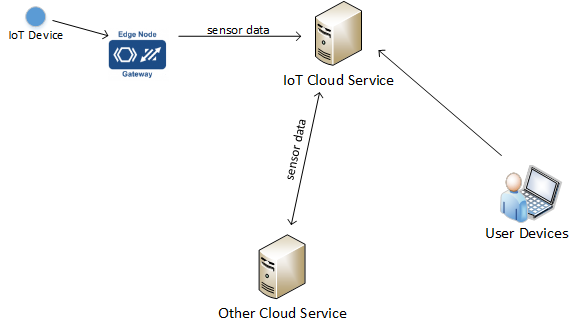
\includegraphics[scale=0.8]{../02_Analyse/images/cloudservices.png}
\caption{IoT-Cloud-Service Übersicht}
\end{figure}

Wie in der Einführung bereits erwähnt, können die Folgen von Ausfällen je nach Applikation sehr unterschiedlich sein. Eintrittswahrscheinlichkeiten und Schadensausmasse müssen in einer Risikoanalyse bewertet werden, damit geeignete Massnahmen getroffen werden können. So benötigen Patientensysteme in Spitälern weitaus mehr Sicherheitsmassnahmen als Pflanzenüberwachungssysteme in Gewächshäusern.

\subsection{API-Security}
Kommunikation und Austausch von Daten erfolgen über bereitgestellte APIs. Sämtliche API Zugriffe müssen zuerst authentifiziert werden, ansonsten können möglicherweise geheime Daten abgefragt-, oder gar fehlerhafte und schädliche Inputs eingegeben werden. Mittels Berechtigungen sollte festgelegt werden, wer auf welche Daten zugreifen darf. 

\subsection{Korrektheit}
Je nach Sensitivität der Cloud-Applikation müssen Softwareentwickler ein erhöhtes Augenmerk auf die Korrektheit der Software legen. Die Vergangenheit hat gezeigt, dass Softwarefehler wie falsches Exception Handling oder Race Conditions weitreichende Folgen haben können. Hängt beispielsweise eine ganze Produktionskette von der Cloud-Applikation ab, so könnte ein Absturz innert kürzester Zeit einen sehr hohen finanziellen Schaden bedeuten. 

\subsection{Verfügbarkeit}
Wie bei herkömmlichen Servern muss auch bei Applikationsserver im IoT-Bereich auf die Verfügbarkeit geachtet werden. Es gibt potenziell viele Vorfälle, welche die Verfügbarkeit beeinträchtigen könnten. Als wirksamste Methode empfiehlt sich eine redundante Auslegung der wichtigsten Komponenten.

\section{User-Devices}
In diesem Unterkapitel werden Gefahren und Massnahmen für End-User Devices behandelt. Über Geräte PCs, Notebooks, Tablets oder Smartphones werden IoT-Services konsumiert. Für Unternehmen stellen sich seit dem ''bring-your-own-device''-Zeitalter die Herausforderung, dass nicht nur User Devices im Firmenbesitz auf interne Anwendungen zugreifen. Network-Access-Control-Systeme überprüfen diverse Attribute wie beispielsweise Virendefinitionen von Devices an einem Enforcement-Point, bevor in den geschützten Bereich zugegriffen werden kann. Grundsätzlich unterscheiden sich die empfohlenen Security-Massnahmen für User-Devices für IoT-Anwendungen nicht von herkömmlichen Systemen, da potenzielle Schadensausmasse jedoch höher sind, sollten empfohlene Massnahmen konsequent umgesetzt werden.

\subsection{Client-Applikationen}
Unterschiedliche Arten von Client-Applikationen sind für IoT-Anwendungen denkbar. Herkömmlich installierte Desktop-Programme für Windows-Betriebssysteme verlieren an Bedeutung. Web- und Mobil-Applikationen haben in den letzten Jahren stark zugenommen. 

Ein Benutzer muss sich an der Client-Anwendung authentisieren. Wie hinlänglich bekannt, muss die Authentifizierung an einem vorgesehenen Server stattfinden. Für sensitive Anwendungen sollten Multi-Faktor-Authentifizierungslösungen eingesetzt werden. Neuere Mobilgeräte und Notebooks verfügen häufig über Fingerabdruckscanner, es wären aber auch SMS-Tokens oder Smartcards als weitere Möglichkeit neben Passwörtern denkbar.

Mobile Geräte werden oft verloren oder gestohlen. Sobald eine Session beendet wurde, sollte eine erneute Authentifizierung verlangt werden. Es sollte ein möglichst kurzes Session-Timeout gewählt werden, damit beim Vergessen des Logouts fremde Personen keinen Zugriff erhalten können.

Viele sicherheitsrelevante Überprüfungen von Anwendungen wie Input-Validierung müssen serverseitig implementiert werden, da man clientseitige Security-Checks leicht umgehen kann. Es gibt jedoch Angriffe wie Phishing oder Social Engineering, welche selbst serverseitig nicht abgefangen werden können. Gegen solche Angriffe schützt man sich am besten mit Benutzerschulungen.

\section{Management-Server}
In diesem Abschnitt wird Security für Management Server behandelt. Ziel dieses Projektes ist ein Prototyp eines Management Servers zu erstellen. Es ist wichtig, bereits vorgängig Security fest einzuplanen, da die Kosten für Security-Vorfälle mit der Zeit zunehmen.

\subsection{Bedeutung}
Management Server sind für Unternehmen sicherheitskritische Systeme. Sie gelten als besonders schützenswert, da viele Applikationen und ganze Geschäftsprozesse abhängig sein könnten. Ist der IoT-Management-Server kompromittiert, so erhält der Angreifer eine Komplettübersicht des gesamten IoT-Systems eines Unternehmens. Als Angreifer könnte man dann beispielsweise versucht sein, Devices herunterzufahren, fehlerhafte Konfigurationen einzuspielen, oder sensitive Informationen zu gewinnen.

\subsection{User Interface}
Es muss die Frage gestellt werden, ob Zugriffe aus dem Internet notwendig sind. Allenfalls könnten externe Benutzer über ein Virtual Private Network (VPN) zugreifen. Angreifer aus dem Internet hätten somit keinen direkten Zugriff ausserhalb des Firmennetzwerks.

Da sensitive Informationen wie Kennwörter und weitere Daten übertragen werden, sollte der Netzwerkverkehr (auch firmenintern) verschlüsselt werden. Wird zum Beispiel ein Web-Interface verwendet, so sollte jeglicher Verkehr über das TLS gesicherte HTTPS-Protokoll geschehen. Unverschlüsselte Verbindungen dürfen nicht erlaubt werden.

Inputvalidierung ist bei Applikationen enorm wichtig. Sicherheitsrelevante Validierungen müssen zwingend serverseitig implementiert werden. Durch saubere Input Validierungen werden häufige Angriffe wie Code Injection, XSS und CSRF Attacken verhindert.

\subsection{Devicekommunikation}
Der Management Server kommuniziert über eigene Sessions mit IoT-Devices. Meldet sich ein Device beim Management Server, so muss dieser zuerst überprüfen, ob das Device berechtigt ist, um mit dem Management Server zu kommunizieren. Auf dem Server könnte beispielsweise ein Passwort hinterlegt werden, welches neuen Devices bekannt sein muss. 

Man könnte auf dem Server auch vertrauenswürdige Root Zertifikate hinterlegen. So könnten Clients, welche Zertifikate von einem dieser vertrauten Root Zertifikate ausgestellt erhalten haben auf den Management Server zugreifen. Der lokale Bootstrap-Server könnte solche Clientzertifikate an die IoT-Devices ausstellen.

\begin{figure}[H]
\centering
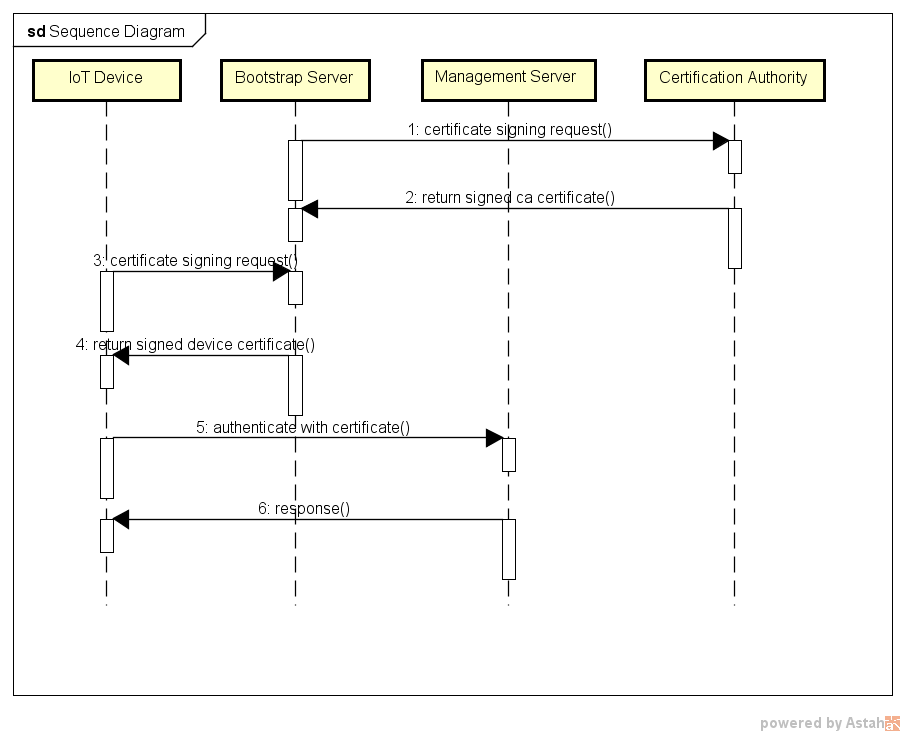
\includegraphics[scale=0.7]{../02_Analyse/images/certificateauthentication.png}
\caption{Authentisierung mit Zertifikaten}
\end{figure}

IoT-Devices übermitteln unter Umständen sensitive Daten an den Management Server. Die Kommunikation muss deshalb verschlüsselt werden.

\subsection{Server}
Die Management Applikation sollte über ein sicheres Authentifizierungsverfahren verfügen. Für kritische Applikationen lohnt sich eine Zwei-Faktor-Authentifizierung. Viele Benutzer verwenden überall die selben Kennwörter oder schreiben sie sich auf, weshalb ein Verlust des Kennworts nicht sehr unwahrscheinlich ist. Durch eine zweite Authentifizierungshürde verbessert sich die Sicherheit markant.

Bereitgestellte APIs müssen geschützt sein. Nur authentifizierte Benutzer sollten zugreifen dürfen. Die Kommunikation über diese APIs muss gesichert sein, dass keine schädlichen Daten übertragen werden können. 

Auch für Management Server ist die Verfügbarkeit wichtig. Hardwarekomponenten sollten redundant vorhanden sein. Der Applikationsserver sollte regelmässig gesichert sein, sodass im Totalausfall durch einen Restore die Downtime möglichst kurz gehalten wird.




